\begin{frame}[fragile]
	\frametitle{Prerequisites}
	\framesubtitle{BWT Transform: Pseudocode}
	Assuming our strings' indices are 1-based, we now give a non-efficient algorithm to calculate
	the BWT transform of a string.
	\begin{minted}[numbersep=5pt,
			frame=lines,
			framesep=2mm]{python}
def BWT(s: str) -> str:
	T = []
	for character in s:
		s = s[len(s)] + s[1..len(s)-1]
		T.push(s)
	sort_lexicographically(T)
	return last_column(T)
	\end{minted}
\end{frame}

\begin{frame}
	\frametitle{Prerequisites}
	\framesubtitle{BWT Transform: Example}
	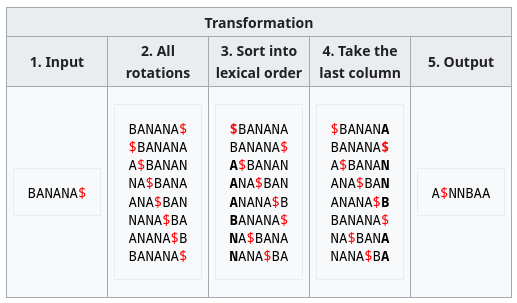
\includegraphics[scale=0.56]{images/bwt-example.png}
\end{frame}

\begin{frame}
	\frametitle{Prerequisites}
	\framesubtitle{Elastic Founder Graph: Block graph}
	\begin{definition}[Block Graph]
		We call \textbf{block graph} an undirected graph in which every biconnected
		component (i.e. a \textbf{block}) is a clique.
	\end{definition}
	\begin{center}
		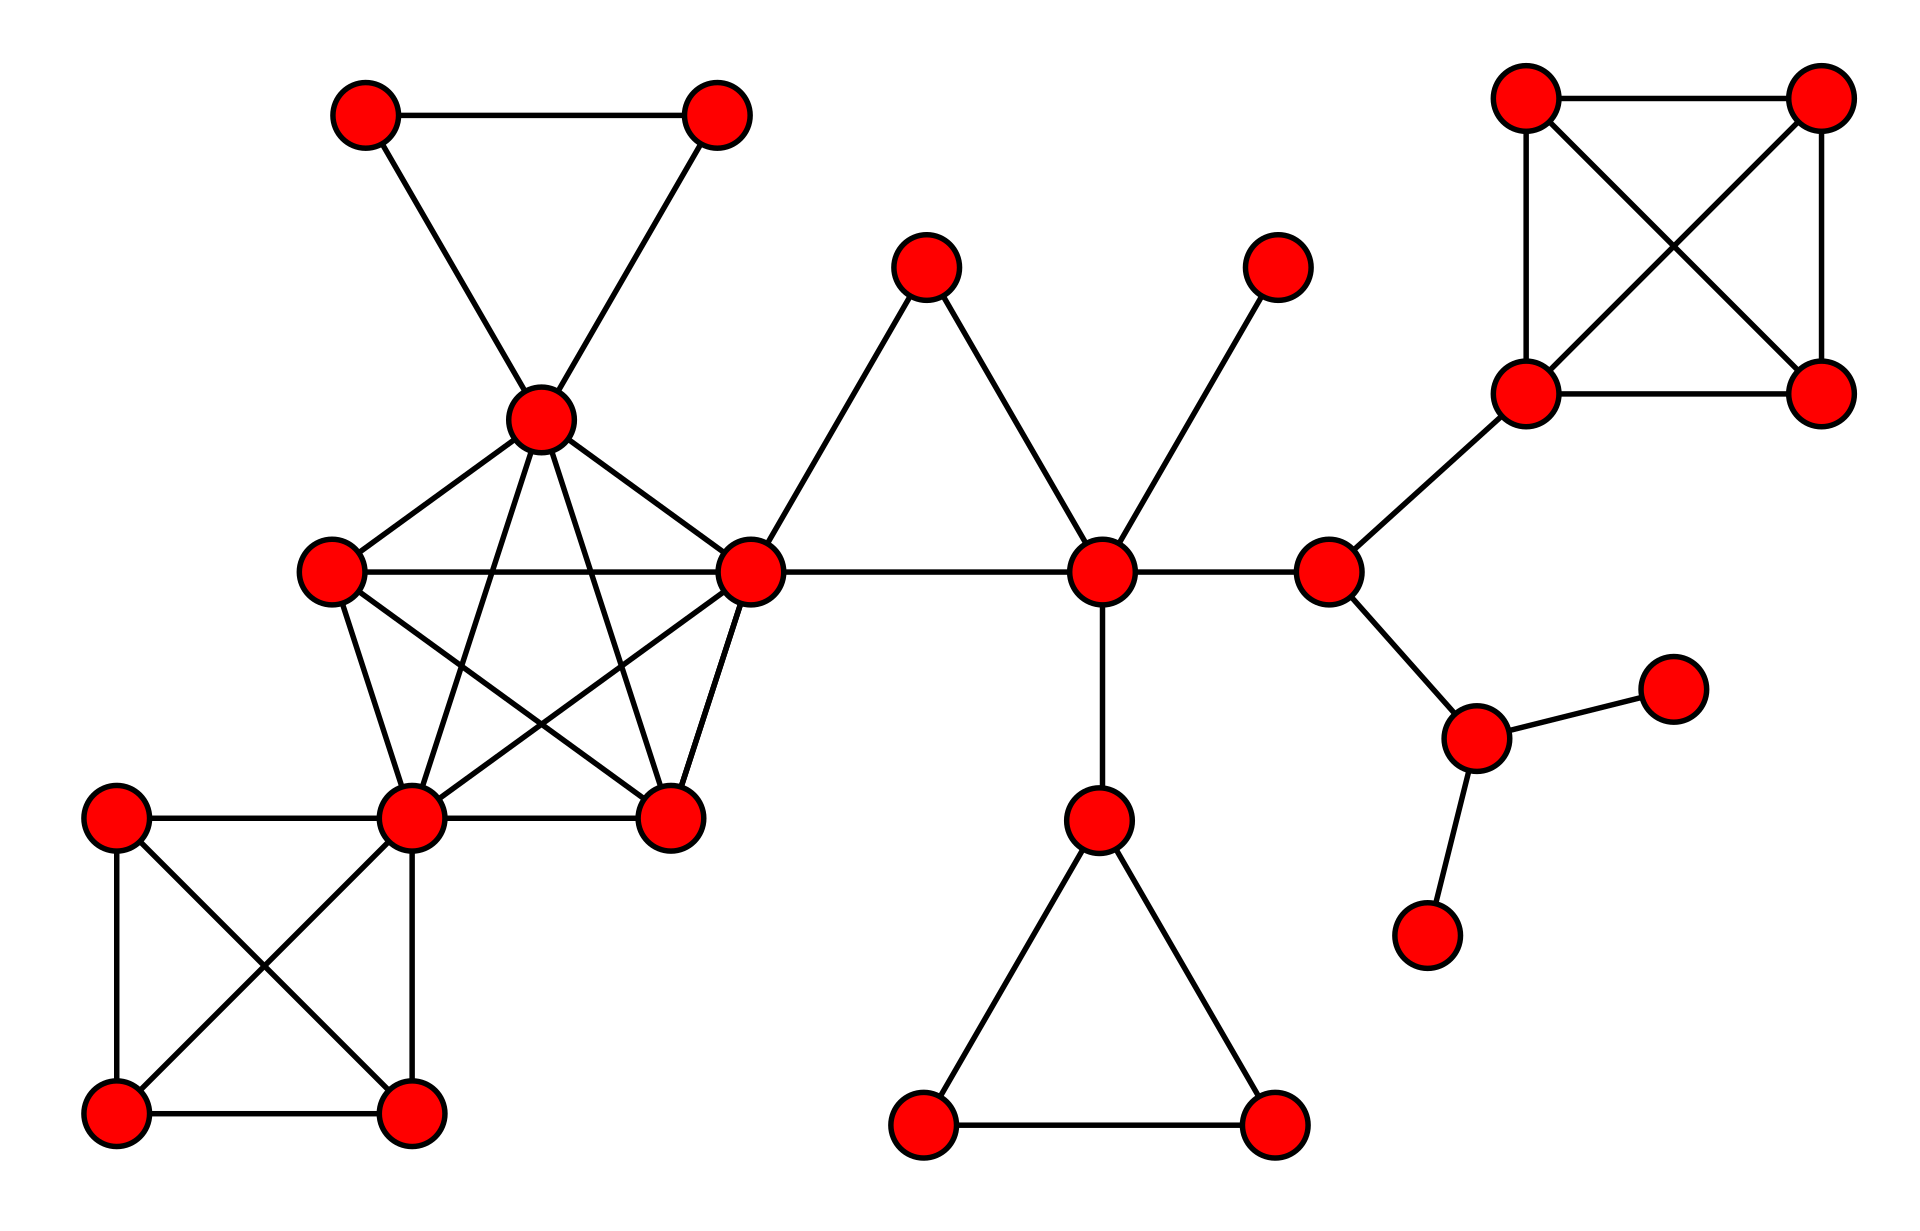
\includegraphics[scale=0.09]{images/block_graph.png}		
	\end{center}
\end{frame}

\begin{frame}
	\frametitle{Prerequisites}
	\framesubtitle{Elastic Founder Graph: definition}
	\begin{definition}[Elastic Founder Graph]
		Consider a block graph \(G = (V, E, l)\) with \(l: V \rightarrow \Sigma^+\). We call such a graph
		an \textbf{indexable Elastic Founder Graph} if the \textbf{semi-repeat-free} property holds: for each
		\(v\) in block \(V_i\), \(l(v)\) occurs in \(G\) only as prefix of paths starting with some
		\(w \in V_i\).
	\end{definition}
\end{frame}